\chapter{Kiểm thử và đánh giá}

\section{Cách kiểm thử}

Nhóm kiểm thử theo bốn mức, từ nhanh và rẻ đến sát thực tế (Bảng~\ref{tab:mucthu}).

\begin{table}[H]
\centering
\caption{Các mức kiểm thử}
\label{tab:mucthu}
\begin{tabularx}{\textwidth}{@{}P{3.4cm}LP{3.6cm}@{}}
\toprule
\textbf{Mức} & \textbf{Phạm vi} & \textbf{Công cụ} \\ \midrule
1. Kiểm thử nghiệp vụ & Toàn bộ phần xử lý trên Lambda: cho vào, cho ra, biển số demo, tính tiền, bỏ tin trùng, phân quyền, email, ghi nhớ email, dọn dữ liệu. Chạy trên DynamoDB giả lập nên không tốn tiền AWS & \code{pytest}, \code{moto} \\
2. Kiểm thử phần phát hiện xe & Phát hiện vật so với nền, mỗi lần đưa tay một lượt, bỏ qua thay đổi ánh sáng, hiện danh sách xe & \code{unittest} trên Pi \\
3. Tích hợp trên AWS & Thiết bị (mô phỏng, rồi thật) kết nối IoT Core thật; kiểm tra trọn luồng qua API và web thật & Chương trình mô phỏng, trang web \\
4. Chạy với thiết bị thật & Pi, ESP32-S3 điều khiển cần chắn, ESP32 18 nút đều kết nối AWS & Trang camera, log của bo mạch \\
\bottomrule
\end{tabularx}
\end{table}

\section{Kiểm thử nghiệp vụ}

Tệp \code{backend/\allowbreak{}tests/\allowbreak{}test\_\allowbreak{}flow.py} gọi thẳng các hàm Lambda với tin nhắn MQTT và yêu cầu API giả, rồi kiểm tra dữ liệu trong DynamoDB giả lập. Kết quả: 16/16 kịch bản đạt (\code{16 passed in 4.13s}).

\begin{longtable}{@{}P{5.2cm}P{6.6cm}P{1.6cm}P{0.8cm}@{}}
\caption{Kết quả kiểm thử nghiệp vụ}\label{tab:unittest}\\
\toprule
\textbf{Kịch bản} & \textbf{Nội dung kiểm tra} & \textbf{SIM} & \textbf{KQ} \\ \midrule
\endfirsthead
\toprule
\textbf{Kịch bản} & \textbf{Nội dung} & \textbf{SIM} & \textbf{KQ} \\ \midrule
\endhead
\code{slots\_\allowbreak{}unknown\_\allowbreak{}until\_\allowbreak{}snapshot} & Ô ở trạng thái không rõ cho tới khi nhận trạng thái đầu tiên & -- & Đạt \\
\code{entry\_\allowbreak{}and\_\allowbreak{}exit\_\allowbreak{}need\_\allowbreak{}admin} & Xe vào thì chờ cho vào, biển 11111, 22222, cần chưa mở. Cho vào thì mở cần, xe vào danh sách. Từ chối một lượt thì xe sau nhận lại số đó. Ô gợi ý đổi theo nút ô. Xe ra là xe số lớn nhất; miễn phí vẫn chờ \emph{Cho ra}; cho ra thì mở cần và xe rời danh sách & 01, 02, 07, 09 & Đạt \\
\code{exit\_\allowbreak{}with\_\allowbreak{}empty\_\allowbreak{}lot} & Bãi trống mà camera báo xe ra thì bỏ qua & 13 & Đạt \\
\code{paid\_\allowbreak{}exit\_\allowbreak{}requires\_\allowbreak{}admin} & Có phí thì chưa cho ra. Miễn phí mà không ghi lý do thì báo lỗi. Ghi đã thu thì mở cần, kết thúc phiên & 07 & Đạt \\
\code{replay\_\allowbreak{}and\_\allowbreak{}full} & Gửi lặp cùng mã sự kiện không tạo lượt thứ hai. Bãi đầy thì không cho vào, không mở cần & 10, 06 & Đạt \\
\code{wrong\_\allowbreak{}lane\_\allowbreak{}is\_\allowbreak{}ignored} & Tin sai làn bị bỏ qua. Biển đọc được nhưng không có trong bãi cũng bỏ qua & 08 & Đạt \\
\code{remember\_\allowbreak{}email\_\allowbreak{}for\_\allowbreak{}plate} & Tích ghi nhớ thì email có link hủy. Xe ra rồi vào lại thì tự gửi email. Hủy bằng link thì xóa liên kết. Link giả thì báo không tìm thấy & 04 & Đạt \\
\code{forget\_\allowbreak{}email\_\allowbreak{}from\_\allowbreak{}qr\_\allowbreak{}page} & Nút bỏ liên kết trên trang QR xóa liên kết & 04 & Đạt \\
\code{slots\_\allowbreak{}offline\_\allowbreak{}still\_\allowbreak{}lets\_\allowbreak{}cars\_\allowbreak{}in} & Bo mạch ô mất kết nối thì ô thành không rõ; xe vẫn được cho vào, chỉ không có ô gợi ý & 11 & Đạt \\
\code{email\_once} & Không tích đồng ý thì báo lỗi. Gửi thành công kèm ô đã chọn. Gửi lại cùng khóa chống lặp thì không gửi lần hai. Khóa khác thì báo đã gửi. Link bị sửa thì báo không tìm thấy & 03, 15 & Đạt \\
\code{permissions} & Tài khoản màn hình ở cổng gọi API quản trị thì bị từ chối; chưa đăng nhập thì báo lỗi & -- & Đạt \\
\code{fee\_table} & 14, 15, 60, 61, 120, 121 phút cho ra 0; 10.000; 10.000; 15.000; 15.000; 20.000 đ & 07 & Đạt \\
\code{gate\_\allowbreak{}ack\_\allowbreak{}timeout} & Lệnh chờ phản hồi được xóa khi cổng báo đã mở & 12 & Đạt \\
\code{duplicate\_plate} & Biển số đang trong bãi không được cho vào lần hai & 09 & Đạt \\
\code{ses\_\allowbreak{}failure\_\allowbreak{}keeps\_\allowbreak{}session} & SES báo lỗi (gửi tới địa chỉ chưa xác minh): phiên đỗ vẫn bình thường, ghi gửi thất bại, có cảnh báo, khách vẫn xem được đường đi & 14 & Đạt \\
\code{purge\_\allowbreak{}after\_\allowbreak{}ten\_\allowbreak{}days} & Dữ liệu đã quá 10 ngày: tác vụ dọn dữ liệu xóa biển số, email, mã QR; biển số không còn bị khóa & 16 & Đạt \\
\bottomrule
\end{longtable}

\section{Kiểm thử phần phát hiện xe trên Pi}

5/5 kiểm thử đạt, chạy cả trên Pi (Python 3.13) và trên máy phát triển:
\begin{itemize}
  \item Giữ ``tay'' trong khung 20 khung hình liên tiếp chỉ tạo \emph{một} lượt. Rút ra rồi đưa lại thì tạo lượt mới.
  \item Nhiễu 2 khung hình không tạo lượt.
  \item Cả khung sáng lên không bị coi là có xe.
  \item Vật nằm yên quá lâu được tính vào nền.
  \item Danh sách xe nhận từ đám mây được hiện đúng.
\end{itemize}

\section{Kiểm thử tích hợp trên AWS}

\subsection{Chạy với thiết bị thật}\label{sec:vong2}

Pi nối dây LAN với laptop (laptop chia sẻ Internet). ESP32-S3 điều khiển cần chắn và ESP32 đọc 18 nút nối Wi-Fi 2,4~GHz. Kết quả:

\begin{enumerate}
  \item Cả ba thiết bị \code{pi-01}, \code{gate-01}, \code{slots-01} đều kết nối. Bo mạch ô gửi trạng thái ``18 ô (0 có xe)''; sơ đồ trên web hiện 18 ô trống.
  \item Bấm \emph{Thử xe VÀO} trên trang camera: đám mây tạo phiên chờ cho vào với biển 33333 (lúc đó 11111, 22222 đã trong bãi). Trang camera nhận được danh sách ``Trong bãi: 11111, 22222 / Chờ cho vào: 33333''.
  \item Nhân viên bấm \emph{Cho vào} hoặc \emph{Cho ra}: ESP32-S3 nhận lệnh, servo quay 180° (vào) hoặc 0° (ra), sau 5 giây về 90°, và báo lại đủ các bước. Danh sách xe trên web và trên Pi cập nhật theo.
  \item Trang QR gợi ý ô trống; chọn ô tầng 2 thì đường đi vẽ lên dốc (Hình~\ref{fig:qr}). Email hướng dẫn gửi được; email tự gửi theo biển số đã ghi nhớ hoạt động; link hủy chạy đúng.
\end{enumerate}

Hai lỗi phát hiện khi chạy thật đã được sửa (Bảng~\ref{tab:suco}): ESP32 bị AWS ngắt mỗi 2 giây vì đăng ký kênh rỗng, và servo không quay vì chân \code{5Vin} của ESP32-S3 không có điện.

\begin{figure}[H]
\centering
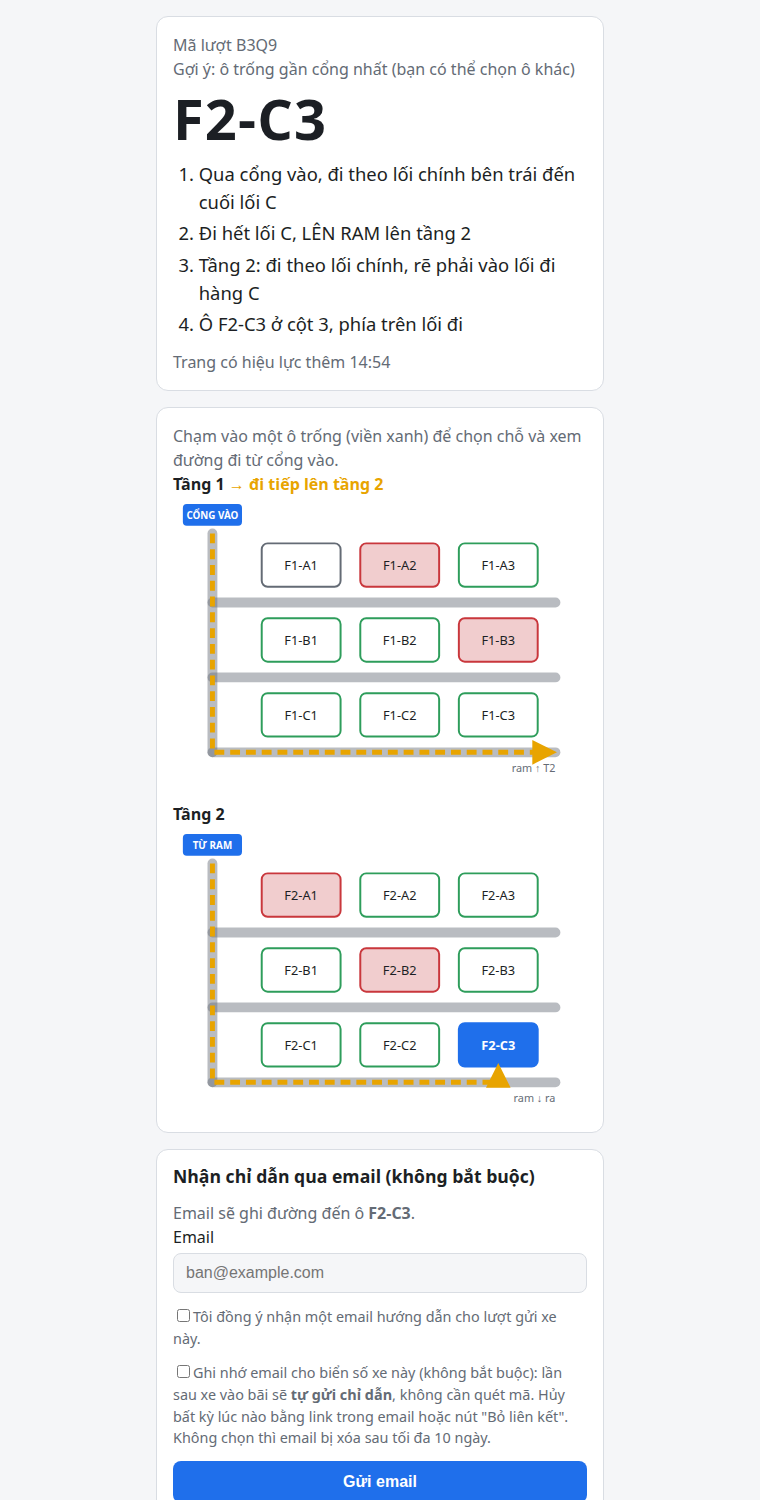
\includegraphics[width=0.5\textwidth]{hinh/web-qr-duongdi.png}
\caption{Trang của khách: gợi ý ô F2-C3, đường đi lên tầng 2 và ô nhập email (chạy với dữ liệu mẫu)}
\label{fig:qr}
\end{figure}

\section{Kiểm thử với camera thật}\label{sec:camthat}

Camera OV5647 trên Pi 5, hai vùng làn là hai nửa khung hình. Kết quả quan sát:
\begin{itemize}
  \item Làn trống: tỉ lệ khác nền gần 0\,\% ở cả hai làn, không gửi sự kiện nhầm.
  \item Đưa tay vào làn: tỉ lệ khác nền vượt ngưỡng 8\,\%, khung làn đổi màu, gửi \emph{đúng một} sự kiện cho mỗi lần đưa tay. Giữ tay lâu không tạo thêm lượt.
  \item Đổi góc camera: bấm \emph{Chụp lại nền} khi làn trống thì phát hiện chạy lại bình thường.
\end{itemize}
Có lần camera chỉ gửi được một khung hình rồi treo, do cáp camera cắm lỏng; cắm lại thì chạy bình thường. Nút \emph{Thử xe VÀO}, \emph{Thử xe RA} trên trang camera gửi đúng loại tin nhắn như camera, nên cũng dùng được để kiểm tra phần còn lại của hệ thống.

\section{Bảng nghiệm thu theo kịch bản}

\begin{longtable}{@{}P{1.3cm}P{7.4cm}P{3.1cm}P{2.3cm}@{}}
\caption{Kết quả nghiệm thu SIM-01 đến SIM-16}\label{tab:nghiemthu}\\
\toprule
\textbf{Mã} & \textbf{Kịch bản} & \textbf{Kiểm bằng} & \textbf{Kết quả} \\ \midrule
\endfirsthead
\toprule
\textbf{Mã} & \textbf{Kịch bản} & \textbf{Kiểm bằng} & \textbf{Kết quả} \\ \midrule
\endhead
SIM-01 & Đưa tay vào làn vào: một phiên chờ cho vào, biển 11111, cần chưa mở & Mức 1, mức 4 & Đạt \\
SIM-02 & Nhân viên \emph{Cho vào}: cần quay trái rồi về giữa, xe vào danh sách (web và Pi), màn hình ở cổng có QR & Mức 1, mức 4 & Đạt \\
SIM-03 & Chọn ô tầng 2 trên trang QR, nhập email: đường đi lên dốc; một email đúng ô & Mức 1, mức 3 & Đạt \\
SIM-04 & Ghi nhớ email: lần sau tự gửi; hủy liên kết thì không gửi & Mức 1, mức 3 & Đạt \\
SIM-05 & Nút ô đảo trạng thái, giữ được sau khi khởi động lại, không đổi phiên đỗ & Bo mạch thật & Đạt \\
SIM-06 & Bãi đầy: không cho vào, không mở cần & Mức 1 & Đạt \\
SIM-07 & Xe ra: chọn xe số lớn nhất, hiện số tiền; chỉ mở cần khi nhân viên cho ra (có phí thì sau khi thu); xe rời danh sách & Mức 1, mức 4 & Đạt \\
SIM-08 & Giữ tay lâu, rút ra đưa lại: mỗi lần đưa tay đúng một lượt & Mức 2, mức 4 & Đạt \\
SIM-09 & Hai lượt chờ vào nhận biển khác nhau; từ chối một lượt thì số được dùng lại & Mức 1 & Đạt \\
SIM-10 & Gửi lặp cùng mã sự kiện, mã lệnh & Mức 1, mô phỏng cổng & Đạt \\
SIM-11 & Bo mạch ô mất kết nối quá 90 giây: ô thành không rõ, xe vẫn được cho vào & Mức 1 & Đạt \\
SIM-12 & Lệnh cũ gửi tới sau khi cổng kết nối lại bị bỏ qua & Mô phỏng cổng & Đạt \\
SIM-13 & Camera báo xe ra khi bãi trống: bỏ qua & Mức 1 & Đạt \\
SIM-14 & SES gửi lỗi: vẫn chỉ đường, ghi gửi thất bại & Mức 1 & Đạt \\
SIM-15 & Link sai hoặc hết hạn, gửi email lần hai & Mức 1 & Đạt \\
SIM-16 & Dữ liệu định danh quá 10 ngày bị ẩn và xóa & Mức 1, chạy tác vụ trên AWS & Đạt \\
\bottomrule
\end{longtable}

\section{Đánh giá}

\subsection{Mức đáp ứng yêu cầu}

Luồng chính chạy được trên AWS với thiết bị thật: xe vào (chờ cho vào, nhân viên cho vào), chỉ đường, xe ra (chờ cho ra, thu tiền, cho ra). Cả 16/16 kịch bản nghiệm thu đều đạt.

\subsection{Số liệu đo}

\begin{table}[H]
\centering
\caption{Số liệu đo trên hệ thống thật}
\label{tab:solieu}
\begin{tabularx}{\textwidth}{@{}LP{5.6cm}@{}}
\toprule
\textbf{Chỉ số} & \textbf{Kết quả} \\ \midrule
Thời gian từ lúc gửi sự kiện có xe tới khi đám mây xử lý xong (10 lần đo ngày 27/11/2026, gửi từ laptop ở Hà Nội tới vùng Singapore) & Trung vị 0,22 giây; nhỏ nhất 0,20 giây; lớn nhất 1,99 giây (lần đầu, Lambda khởi động nguội) \\
Số kịch bản nghiệm thu đạt & 16/16 \\
Số kiểm thử tự động đạt & 16/16 (đám mây), 5/5 (Pi) \\
Chi phí AWS thực tế từ 1/11 đến 27/11/2026 (theo AWS Cost Explorer) & Khoảng 0,09 USD, đã được tín dụng trừ hết. Nhiều nhất là DynamoDB (0,046 USD) và API Gateway (0,016 USD) \\
\bottomrule
\end{tabularx}
\end{table}

Thời gian xử lý đáp ứng NFR-07 (dưới 2 giây). Chi phí thực tế thấp hơn nhiều so với ước tính ở Bảng~\ref{tab:chiphi}, vì hệ thống chỉ chạy vài giờ mỗi ngày để làm demo.

\subsection{Hạn chế}

\begin{itemize}
  \item Camera chỉ phát hiện ``có vật'' trong làn, không đọc biển số. Biển số là số demo do hệ thống cấp. Xe ra luôn là xe có số lớn nhất, nhân viên không chọn được xe khác.
  \item Biển số demo được dùng lại cho xe sau. Vì vậy email đã ghi nhớ theo một biển demo sẽ được gửi cho lượt sau; cần bỏ liên kết sau khi demo.
  \item 18 ô dùng nút nhấn giả lập cảm biến, chưa chứng minh được việc phát hiện xe thật. Bãi đầy chỉ tính theo nút ô.
  \item Không có cảm biến xe qua cổng, nên mọi lượt vào, ra cần nhân viên bấm cho phép.
  \item SES đang ở chế độ thử, chỉ gửi được tới địa chỉ đã xác minh.
\end{itemize}
